% Draft preprint. Numbers come from the committed outputs in ../ and can be regenerated with the
% score.py scripts there and figures/make_figures.py. Build: pdflatex, bibtex, pdflatex, pdflatex.
\documentclass[11pt]{article}
\usepackage[utf8]{inputenc}
\usepackage[margin=1in]{geometry}
\usepackage{graphicx,booktabs,xcolor}
\usepackage[numbers,sort&compress]{natbib}
\usepackage[colorlinks=true,linkcolor=blue,citecolor=blue,urlcolor=blue]{hyperref}
\setlength{\parindent}{0pt}\setlength{\parskip}{6pt plus 2pt minus 1pt}
\newcommand{\todo}[1]{\textcolor{red}{[TODO: #1]}}

\title{Two recent Claude models read catalytic residues, domains and secondary structure from protein sequence alone}
% TODO: confirm the author list, affiliations and corresponding author before posting.
\author{Christopher J. Mungall \todo{confirm authors and affiliations}}
\date{Draft of 19 November 2026}

\begin{document}
\maketitle

\begin{abstract}
A recent report showed that two general-purpose language models, Claude Fable~5.2 and Claude Opus~5.5,
predict the next residue of obscure proteins far better than chance. We ask whether that ability is useful
for annotation. Given only an amino-acid sequence and no tools, both models named the correct Pfam family
for 35 to 39 of 45 sampled bacterial and archaeal proteins, with domain boundaries overlapping the
reference by 0.85, and almost never assigned a domain to a shuffled sequence. They detected a single
catalytic-residue substitution introduced into an active kinase: a catalytic aspartate-to-asparagine mutant
was called active in 0 of 20 cases by either model, against 18 of 20 for the older Claude Opus~4.6, which
was run at a lower effort setting. For recently released protein structures with no earlier PDB entry at
30\% sequence identity or more, three-state secondary structure accuracy was 73 to 76\%, against 57\% for
the best single-state guess, and long-range contact precision was 19 to 37\%, against 2\% by chance. The models also fail in specific ways: they shift a catalytic role to a neighbouring identical
residue, and they argue around a substitution they have just reported. The tests are small, each
question was asked once, and only models from one vendor were tested. We conclude that sequence-only reading by these models is good enough to triage
pseudoenzyme over-annotation, and is not a citable source of evidence.
\end{abstract}

\section{Introduction}

Protein language models such as ESM-2 and ProtGPT2 learn sequence statistics from protein databases and
support structure prediction and design \citep{lin2023esm2,ferruz2022protgpt2}. General-purpose language
models are trained for other purposes. Tu and Chen recently reported that two of them nevertheless carry
sequence knowledge: on proteins from little-studied domain-of-unknown-function families, Claude Fable~5.2
and Claude Opus~5.5 predicted the next amino acid much more often for real sequences than for shuffled
ones, at a level comparable to dedicated protein language models. The same report found little or no such
signal in the models it tested from other vendors, and a smaller one in earlier Claude models
\citep{tu2026claude,tu2026probe}. Our tests cover the two models with the strongest reported signal and one
earlier Claude model, and say nothing about language models in general.

Next-residue accuracy does not say whether a model can do anything a curator needs. Function prediction
tools make characteristic errors, and one of the most damaging is to assign a catalytic activity to a
protein that keeps the fold of an enzyme and has lost its catalytic residues
\citep{decrecy2025limitations}. Pseudokinases are the best-known case \citep{kwon2019pseudokinases}. A
model that only recognises the family will repeat this error; a model that reads the residues should not.

We therefore ran four small tests, each with a control the model could not pass by recall: a subsample
replication of the next-residue result; domain and membrane-feature annotation with shuffled sequences as
a control; catalytic-activity calls on kinases carrying a single substitution that we introduced; and
secondary structure, contact and function prediction for structures released in the PDB in the three
months before the tests.

\section{Methods}

\paragraph{Models and access.} We tested \texttt{claude-fable-5-2}, \texttt{claude-opus-5-5} and, as an
older comparison, \texttt{claude-opus-4-6}. Each question was one call to the \texttt{claude} command-line
tool in print mode with no tools and an empty system prompt; we confirmed that calls were single-turn with
no web search or fetch. This route does not expose temperature, so answers were sampled, and it adds about
1,400 tokens of its own context. Fable~5.2 and Opus~5.5 ran at high effort in tests 2 to 4. Opus~4.6 ran at
low effort because it did not finish at high effort, so comparisons with it are confounded by effort.
Each question was asked once. For 6 of the 2,570 calls, the tool's usage record lists a second model
besides the one requested: three Opus~5.5 next-residue calls at high effort, all on shuffled sequences, and
in test 4 one Fable~5.2 and two Opus~5.5 calls, all on known-stratum entries. One of the Opus~5.5 test-4
calls (PDB 7IMP) returned an API error instead of an answer and is excluded from the scores; for the other
five, the record does not show which model wrote the answer, and they are kept in the reported numbers;
the repository gives tests 1 and 4 with them excluded, and no conclusion changes.
Where a reply held more than one JSON object, we scored the last one; this applies to three Opus~4.6
replies in test 2, in which the second object corrects the first. One Opus~5.5 next-residue reply was a
written-out web request instead of a prediction; it is counted as invalid and as a wrong answer.

\paragraph{Test 1, next residue.} We drew 68 of the 167 families in the public test set
\citep{tu2026probe} (17 per family-size bin), one protein per family and two of its five cut points, and
used the authors' prompt unchanged. The model writes the next ten residues and the first is scored.
Controls were the same protein shuffled with the authors' seed and, new here, the real sequence reversed.
Intervals are 95\% bootstrap intervals over families.

\paragraph{Test 2, domains and membrane features.} The test set was 45 unreviewed bacterial and archaeal
UniProt entries of 150 to 450 residues with a Pfam match, drawn haphazardly through the search interface
\citep{uniprot}, and 15 proteins from the test set of \citep{tu2026probe}. The model returned Pfam domains
with coordinates \citep{mistry2021pfam}, transmembrane helices, a signal-peptide call, a name and a
function. Truth was the InterPro Pfam matches and the UniProt transmembrane and signal features, which in
unreviewed entries are themselves predicted. Each protein was also presented shuffled.

\paragraph{Test 3, pseudoenzymes.} From Swiss-Prot, excluding human, mouse and rat, we took 20 active
protein kinases with a curated proton-acceptor aspartate and ATP-binding lysine; 20 kinase-fold proteins
whose name contains ``inactive''; and 20 non-kinase enzymes with a curated active site. Each kinase was
also presented with the aspartate changed to asparagine and, separately, the lysine changed to
methionine; each other enzyme with its first active-site residue changed to alanine. One prompt, used for
every sequence, asked for the catalytic residues present, any that were substituted or missing, and
whether the protein is catalytically active.

\paragraph{Test 4, structure and function.} From the PDB \citep{rcsb} we took X-ray entries released on
or after 1 August 2026 with one protein entity of 100 to 350 residues and resolution of 2.5~\AA{} or
better. We kept 15 entries for which a sequence search found no PDB entity at 30\% identity or more
released before 1 June 2026, and 15 entries with at least 20. We call these strata ``novel'' and ``known''
for short. The labels describe that criterion only. Novel entries may have more distant homologs in the
PDB; 8 of the 12 distinct novel proteins have UniProt accessions, so their sequences were public earlier;
structures are deposited months before release; and the work behind an entry may have been described in
a preprint. We do not know the models' training cutoffs, and the two dates are our assumption that
structures released from August 2026 were not in training. The model predicted helix
and strand ranges, a fold, 20 residue pairs at least 24 apart in sequence that it expected to lie within
8~\AA{} (C$\alpha$), a function, and whether it recognised the sequence as a specific known protein. Truth was the deposited coordinates and the depositors' helix and
sheet records, scored over resolved residues. One protein, human ASPRV1, was drawn four times in the novel
set; we report results with it counted once (12 novel proteins). The function call for those 12 proteins was graded once, unblinded, against the
deposited title by the AI agent that ran the tests.

\section{Results}

\subsection{The next-residue result replicates in direction}

Fable~5.2 predicted real sequence better than shuffled sequence at both effort settings, and Opus~5.5 did
so at high effort; at low effort the interval for Opus~5.5 includes zero. Opus~4.6, run at low effort only,
showed no difference (Table~\ref{tab:next}). Accuracy was well below the published values for the identical questions (58.8\%
for Fable~5.2 and about 40\% for Opus~5.5), which we attribute, without having tested it, to sampled
answers and the extra context. Reversed sequence, tested at low effort only, scored like shuffled
sequence for Fable~5.2 and between shuffled and real for Opus~5.5. Four no-model heuristics,
such as repeating the last residue, scored 7 to 10\% on real, shuffled and reversed sequence alike over
all 3,340 cut points.

Accuracy on real sequence rose with the effort setting. For Fable~5.2 the same 136 real cut points gave
25.0\% at low effort and 41.2\% at high effort, where every answer used thinking tokens; shuffled sequence
gave 7.4\% and 11.8\%. This is the only controlled evidence here on reasoning, and it differs from the
original report, in which answers without thinking were as accurate as those with it.

Within a run, answers that used thinking were more often right, but the model chooses when to think, so
this comparison is descriptive and not a measure of what thinking does. At low effort Fable~5.2 thought on
38 of 136 real cut points and was correct on 57.9\% of them, against 12.2\% of the other 98. It thought on
only 15 shuffled and 17 reversed cut points, and on shuffled sequence thinking did not help (0 of 15
correct, against 10 of 121 without). At high effort, where it thought on every question, its accuracy on
real sequence was 41.2\%, well below the 57.9\% of the questions it had selected itself. The model
appears to think when it recognises something, so the split partly sorts questions by difficulty.
Opus~5.5 at high effort was correct on 39.0\% of real cut points with thinking (41) and 9.9\% without
(91). The reasoning text is not available to us.

\begin{table}[ht]
\centering\small
\caption{Next-residue accuracy on a 68-family subsample. Gap is real minus shuffled, in percentage points,
with a 95\% bootstrap interval over families. The Opus~5.5 high-effort run covers 132 of 136 questions.}
\label{tab:next}
\begin{tabular}{llrrrl}
\toprule
Model & Effort & Real & Shuffled & Reversed & Gap (95\% interval) \\
\midrule
Fable 5.2 & low & 25.0\% & 7.4\% & 8.8\% & $+17.6$ ($+9.6$ to $+26.5$) \\
Fable 5.2 & high & 41.2\% & 11.8\% & -- & $+29.4$ ($+18.4$ to $+40.4$) \\
Opus 5.5 & low & 16.9\% & 9.6\% & 12.5\% & $+7.4$ ($-1.5$ to $+16.2$) \\
Opus 5.5 & high & 18.9\% & 7.6\% & -- & $+11.4$ ($+3.0$ to $+20.5$) \\
Opus 4.6 & low & 5.1\% & 7.4\% & 5.9\% & $-2.2$ ($-7.4$ to $+2.9$) \\
\bottomrule
\end{tabular}
\end{table}

\subsection{Domains and membrane features are recovered, and shuffled sequences are left blank}

Fable~5.2 and Opus~5.5 named at least one correct Pfam family for 39 and 35 of the 45 sampled proteins,
with boundaries close to the reference (mean overlap 0.85 for both, over the correctly named domains in these proteins;
Table~\ref{tab:feat} pools all 60). Fable~5.2 also named the exact family for 8
of 15 proteins from obscure domain-of-unknown-function families. Both models declined to annotate
shuffled sequences. Errors were not marked as such: Fable~5.2 assigned one DUF968 protein to a different
family, and both models split helices in multi-pass transporters (85 and 87 predicted against 74
annotated). Two test proteins carry implausible submitter names in UniProt, ``Glycerol dehydrogenase'' on
a 128-residue DUF3119 membrane protein and ``Methylthioribose kinase'' on a DUF7147 protein; neither model
repeated them.

\begin{table}[ht]
\centering\small
\caption{Annotation from sequence alone. IoU is the overlap of predicted and reference domain boundaries
when the family is correct. The first two rows count proteins in each set; the other rows pool both sets,
60 proteins. Three Opus~4.6 replies held two answers and are scored on the second.}
\label{tab:feat}
\begin{tabular}{lrrr}
\toprule
 & Fable 5.2 & Opus 5.5 & Opus 4.6 \\
\midrule
Sampled proteins with a correct Pfam family & 39/45 & 35/45 & 5/45 \\
Obscure DUF proteins with a correct Pfam family & 8/15 & 3/15 & 0/15 \\
Predicted domains with the right accession & 62/70 & 45/51 & 5/23 \\
Boundary overlap (IoU) & 0.86 & 0.86 & 0.61 \\
Transmembrane helices recovered & 74/74 & 74/74 & 51/74 \\
Signal peptide, true / false positives & 9 / 0 & 9 / 0 & 9 / 7 \\
Shuffled sequences given any domain & 1/60 & 0/60 & 5/60 \\
\bottomrule
\end{tabular}
\end{table}

\subsection{A single catalytic substitution is detected}

Both newer models called all 20 wild-type kinases active and none of the 20 aspartate-to-asparagine
mutants (Figure~\ref{fig:pseudo}). Across the 60 mutant sequences they reported the mutated position as
substituted in 57 (Fable~5.2) and 47 (Opus~5.5); Opus~4.6 reported none and called 18 of 20 mutants
active. Opus~5.5 was weaker on the lysine, calling 7 of 20 lysine-to-methionine mutants active.

Natural pseudokinases were called inactive in 18 of 20 cases by both newer models, but in 17 of those 18
answers, for each model, the model's own protein name already said ``inactive'' or ``pseudokinase'', so this set
mostly measures recall of the entry. The exception is informative: both models called \textit{C.~elegans}
kin-32 (Q95YD4), named an inactive tyrosine kinase in Swiss-Prot, active, citing an intact glycine loop,
VAVK lysine, HRD and DFG motifs, all of which are present in the sequence. We did not examine the basis of
the Swiss-Prot name.

Two failure modes recurred. In the first, the model moved the catalytic role to a neighbouring identical
residue: with Glu318 of a glucuronosyltransferase (Q9VLA1) changed to alanine, both models named Glu317
as the catalytic base and called the enzyme active, although Fable~5.2 had named Glu318 in the wild type.
In the second, the model reported the substitution and then argued around it: for the
\textit{Toxoplasma} kinase ROP17 (Q2PAY3), Fable~5.2 noted methionine at the lysine position and proposed
that a nearby lysine would take its place. For two further enzymes (Q08651 and P64636) both models placed
the catalytic residue beside the curated position in wild type and mutant alike; we could not tell from
these data whether the models or the reference positions are right.

\begin{figure}[ht]
\centering
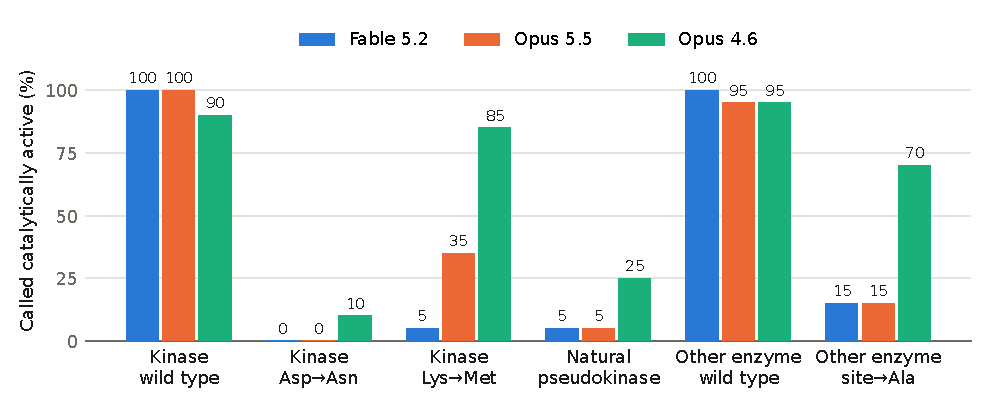
\includegraphics[width=\linewidth]{figures/fig1_pseudoenzyme.pdf}
\caption{Share of sequences called catalytically active, 20 sequences per bar. Mutants carry one
substitution introduced for this study. Opus~4.6 ran at low effort.}
\label{fig:pseudo}
\end{figure}

\subsection{Secondary structure and contacts are predicted above chance for recently released structures}

For the 12 novel proteins, Fable~5.2 and Opus~5.5 reached 76\% and 73\% three-state accuracy, against
57\% for the best single-state guess, and 37\% and 19\% long-range contact precision, against 2\% by
chance (Figure~\ref{fig:struct}). Scores for the known stratum were a few points higher. Fable~5.2 said
it recognised 2 of the 12 novel proteins (ASPRV1 and MrtR) and 14 of the 15 known entries; Opus~5.5 said
it recognised none of the novel proteins. Opus~4.6, at low effort, scored below the single-state guess on
secondary structure and near chance on contacts, which suggests that its low-effort answers say little
about what it can do. These values are far short of dedicated
structure predictors \citep{jumper2021alphafold}; the point is that they are well above chance for a
model given no alignment and no tools.

In the manual grading of function for the 12 novel proteins, Fable~5.2 was correct on 6, abstained on 5
and was wrong on 1; Opus~5.5 was correct on 4, abstained on 7 and was wrong on 1. The correct calls were
mostly members of large, well-characterised families, and we did not test whether the models reached
them through the predicted structure or by recognising the family from sequence. For a domain of
\textit{Arabidopsis} AtDUC1 (PDB 9T71), deposited under the name ``EEIG1/EHBP1 protein amino-terminal
domain protein'', Fable~5.2 predicted a papain-like cysteine peptidase with a Cys-His-Asp triad,
``possibly a deubiquitinase''; the entry is the structure of its deubiquitinase domain. This call cannot
be credited to inference from sequence alone: a preprint describing this protein family as
deubiquitinases was posted in December 2025 \citep{lachmayer2025ducs}, eight months before the structure
was released, and a model trained after that date could have learned it. We did not search for earlier
descriptions of the other novel proteins. The wrong call
from Fable~5.2 was the guanidine prenyltransferase NosH (9TGX), which it named a TenA-family thiaminase.
Neither model identified the RNase~P subunit Rpp30 (10CW) or a designed cysteine protease (9YP0).

One entry gave an unplanned replicate of test 3. One of the ASPRV1 constructs (27IQ) has its catalytic
DSG motif changed to NSG. Both newer models stated, without being asked about activity, that the
catalytic aspartate was replaced and that the construct was probably inactive.

\begin{figure}[ht]
\centering
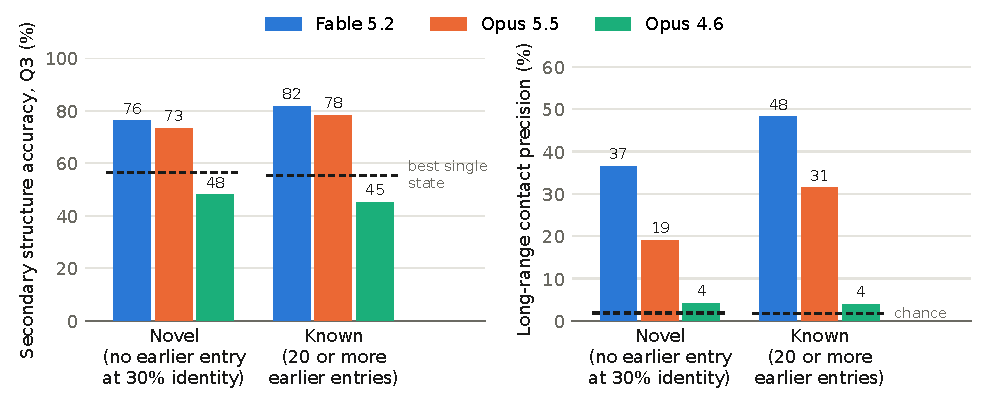
\includegraphics[width=\linewidth]{figures/fig2_structure.pdf}
\caption{Structure prediction from sequence for PDB entries released from August 2026, with ASPRV1
counted once. Novel: no PDB entity at 30\% identity or more released before June 2026. Known: at least 20
such entities. (12 novel, 15 known; for Opus~5.5, the call for one known entry returned an API error instead of an answer). Dashed lines show the best single-state
guess (left) and the chance rate for a long-range pair (right).}
\label{fig:struct}
\end{figure}

\section{Discussion}

Fable~5.2 and Opus~5.5 do more than recognise a family. They change their answer when one catalytic
residue changes and name that residue, and they predict secondary structure and contacts above chance
for proteins with no earlier PDB entry at 30\% identity. How far this extends is not established here. We
tested two models from one vendor. The comparison with Opus~4.6 is not like for like, because it ran at a
lower effort setting, and it is not a blank: at that setting it still found all 9 signal peptides, with 7
false positives, and 51 of 74 transmembrane helices. The report that prompted this work found a graded
next-residue signal across Claude models released between Opus~4.6 and Fable~5.2, and little or none in
other vendors' models \citep{tu2026claude}; we tested none of those, so we cannot say whether reading
catalytic residues tracks that signal.

For annotation review, the practical use is narrow. A sequence-only read can flag a probable pseudoenzyme
before a catalytic term is accepted, and can question an implausible name. It cannot serve as evidence:
the output has no provenance, its errors are stated as confidently as its correct calls, and both failure
modes we observed end in a confident ``active''. A named catalytic position should be checked against the
sequence and a curated feature before it is used.

\paragraph{Limitations.} Cells contain 12 to 68 items, and each question was asked once. Answers were
sampled through a command-line tool that adds its own context, which probably lowers accuracy relative to
direct greedy calls. Opus~4.6 ran at a lower effort setting. Swiss-Prot proteins are well known, so
wild-type results in test 3 may reflect recall; the mutants do not. Transmembrane and signal-peptide truth
in test 2 is predicted. Function in test 4 was graded once, unblinded, by the agent that ran the tests. We did not test eukaryotic
multi-domain proteins in test 2, membrane proteins in test 4, variant effects, or whether reasoning
improves tests 2 to 4. The novel stratum of test 4 excludes close homologs in the PDB and nothing else:
most of its sequences were already public, remote homologs were not excluded, and at least one protein was
described in a preprint before the structure was released. The split of test-1 accuracy by thinking is
observational. We have no information on how these models were trained and draw no conclusion
about it.

\section*{Data and code availability}

Scripts, prompts, test sets and all raw model outputs are at
\url{https://github.com/ai4curation/fable-sequence-to-function}. Every number in this paper is printed by a
scoring script from the committed model outputs, and \texttt{just check} verifies the data checksums and
that the numbers reproduce. Test sets were drawn from live UniProt, InterPro and RCSB services on 18
November 2026 and are committed as drawn, because re-querying those services returns different entries.
Model calls used Claude Code 2.1.327; repeating them will not return identical answers.

\section*{Acknowledgements}

The tests, analysis and first draft were produced by an AI coding agent (Claude Code) under the direction
of the author; the agent is itself built on a Claude model. \todo{funding and other
acknowledgements}

\bibliographystyle{unsrtnat}
\bibliography{references}
\end{document}
